%\usepackage{Paquetes}

\fancyfoot{}
\rfoot{{\small Pág. \thepage}}
\lfoot{{\footnotesize \textbf{Alumnos:} Los mas capos}}
\fancyhead{}
\lhead{{\footnotesize Mecánica de fluidos \\ \textit{UTN - Facultad Regional Reconquista}}}
\rhead{{\footnotesize \textsc{Unidad 1: Propiedades de fluidos}}}
\setlength{\headsep}{1.2cm}

\setlength{\parindent}{0pt}%para sacar la sangría

\section{Unidad 1: Conceptos fundamentales}
\subsection{Definición de fluido y continuo}
Un fluido es aquel que se deforma continuamente cuando se somete a esfuerzos cortantes, por mas mínimos que estos resulten.
\begin{figure}[h]
	\centering
	\begin{subfigure}[b]{0.45\linewidth}
		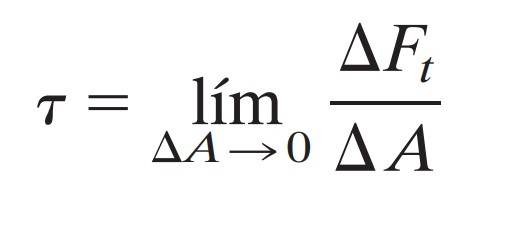
\includegraphics[width= .5\linewidth]{cortante1}
	\end{subfigure}
	\begin{subfigure}[b]{0.45\linewidth}
		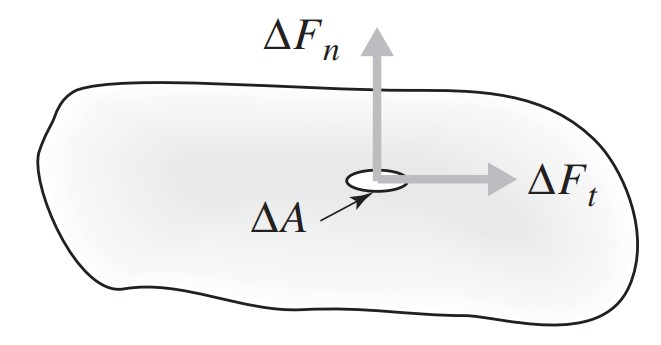
\includegraphics[width= .7\linewidth]{cortante2}
	\end{subfigure}
	\caption{Esfuerzo cortante}
\end{figure}
